\section{Structural Mode Shapes}
In this section, we will describe the cluster-based modal analysis approach with focus on the optimization of clustering. Before we formulate this clustering problem, the basic concept of modal parameters, the techniques adopted for modal analysis and assembling method are described. Table \ref{tab:Table1} summarizes the notations to be used.

\begin{table}
	\centering
\begin{tabular}{|c|l|}
\hline
\(\mathbf{\Psi_k}\)& The \(k^{th}\) mode shape vector of the structure\\
\hline
\(p\) &	The number of mode shape vectors to be identified\\
\hline
\(G_{xy}(\omega)\)& The cross spectral density (\(x\neq y\))\\
\ & and power spectral density (\(x=y\))\\
\hline
\(N\) & the total data amount\\
\hline
\(M,c,n_i\) & the total number of sensor nodes,\\ 
\ & the number of generated clusters, \\
\ & and the number of sensor nodes in cluster \(S_i\)\\
\hline
\(n_t\)	& Length of each section to calculate CSD\\
\hline
\(n_d\)	& Number of averages\\
\hline
\(e_S, e_R, e_T \)& Energy consumed for sampling/rece./trans. one data\\
\hline
\(e_{NExT}, e_{ERA}\)	& Energy consumed for NExT and ERA\\
\hline
\end{tabular}
	\caption{Summary of Notations}
	\label{tab:Table1}
\end{table}

In particular, we give a brief introduction of one important type of modal parameters: mode shapes. 

Each mechanical structure has a number of specific vibration patterns at specific frequencies. These vibration patterns are called mode shapes. For example, we deploy a total of \(m\) sensor nodes on a structure and extract a total of \(p\) mode shapes from the measurement of these sensors:

\begin{equation}
[\mathbf{\Psi_1}, \mathbf{\Psi_2}, \cdots, \mathbf{\Psi_p}]=
\begin{bmatrix}
\phi_{11} & \phi_{12} & \cdots & \phi_{1p}\\
\phi_{21} & \phi_{22} & \cdots & \phi_{2p}\\
\vdots  & \vdots  & \ddots & \vdots  \\
\phi_{m1} & \phi_{m2} & \cdots & \phi_{mp}
\end{bmatrix} 
\end{equation}
where mode shape \(\mathbf{\Psi_k}=[\phi_{1k}, \phi_{2k}, \cdots, \phi_{mk}]'\) is the \(k^{th}\) vibration pattern of the structure.  \(\phi_{ik}(i=1,2,\cdots ,m)\) is the \(k^{th}\) mode shape value defined at the \(i^{th}\) sensor.

As an example, Figure \ref{fig:modes} illustrates the first three mode shapes of a typical cantilevered beam, extracted from the measurements of the deployed 12 sensor nodes. Figure \ref{fig:originalbeam} represents the Original beam. Figure \ref{fig:mode1}, \ref{fig:mode2} and \ref{fig:mode3} represents Mode Shape 1, Mode Shape 2 and Mode Shape 3 respectively.

\begin{figure}
\centering
\subfloat[]{\label{fig:originalbeam}
%\figurecurrentwidth{originalbeam}}
\figurehalfwidth{originalbeam}}
%\qquad
\subfloat[]{\label{fig:mode1}
%\figurecurrentwidth{mode1}}
\figurehalfwidth{mode1}}
\qquad
\subfloat[]{\label{fig:mode2}
%\figurecurrentwidth{mode2}}
\figurehalfwidth{mode2}}
%\qquad
\subfloat[]{\label{fig:mode3}
%\figurecurrentwidth{mode3}}
\figurehalfwidth{mode3}}
%\qquad
%\subfloat[Mode 4 (Freq.=30.8Hz)]{\label{fig:mode4}
%\figurecurrentwidth{mode4}}
%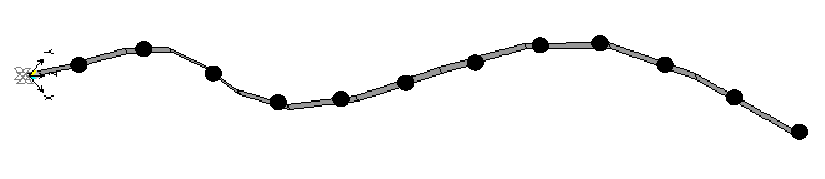
\includegraphics[width=.49\textwidth, height=0.05\textwidth]{mode4}}
\caption{Mode shapes of a typical cantilevered beam}
\label{fig:modes}
\end{figure}

It can be seen that mode shape vector \(\mathbf{\Psi_k}\) has an element corresponding to each sensor node. The more number of sensor nodes used, the more elements are contained in \(\mathbf{\Psi_k}\), and more accurately this vibration pattern of the structure is described. Considering example in Figure \ref{fig:modes}, if we double the number of nodes deployed on the beam, the vibration patterns will be represented with higher granularity. Another important characteristic of mode shape is that elements in \(\mathbf{\Psi_k}\) only represent the relative vibration amplitudes of structure at corresponding sensor nodes. That is, \(\mathbf{\Psi_k}=\zeta \mathbf{\Psi_k}\), where \(\zeta\) is any non-zero real number. This property will be re-visited when we formulate the clustering problem in section \ref{sec:OptimalClustering}.